% Options for packages loaded elsewhere
\PassOptionsToPackage{unicode}{hyperref}
\PassOptionsToPackage{hyphens}{url}
%
\documentclass[
  ignorenonframetext,
  aspectratio=1610,
]{beamer}
\usepackage{pgfpages}
\setbeamertemplate{caption}[numbered]
\setbeamertemplate{caption label separator}{: }
\setbeamercolor{caption name}{fg=normal text.fg}
\beamertemplatenavigationsymbolsempty
% Prevent slide breaks in the middle of a paragraph
\widowpenalties 1 10000
\raggedbottom
\setbeamertemplate{part page}{
  \centering
  \begin{beamercolorbox}[sep=16pt,center]{part title}
    \usebeamerfont{part title}\insertpart\par
  \end{beamercolorbox}
}
\setbeamertemplate{section page}{
  \centering
  \begin{beamercolorbox}[sep=12pt,center]{part title}
    \usebeamerfont{section title}\insertsection\par
  \end{beamercolorbox}
}
\setbeamertemplate{subsection page}{
  \centering
  \begin{beamercolorbox}[sep=8pt,center]{part title}
    \usebeamerfont{subsection title}\insertsubsection\par
  \end{beamercolorbox}
}
\AtBeginPart{
  \frame{\partpage}
}
\AtBeginSection{
  \ifbibliography
  \else
    \frame{\sectionpage}
  \fi
}
\AtBeginSubsection{
  \frame{\subsectionpage}
}
\usepackage{amsmath,amssymb}
\usepackage{iftex}
\ifPDFTeX
  \usepackage[T1]{fontenc}
  \usepackage[utf8]{inputenc}
  \usepackage{textcomp} % provide euro and other symbols
\else % if luatex or xetex
  \usepackage{unicode-math} % this also loads fontspec
  \defaultfontfeatures{Scale=MatchLowercase}
  \defaultfontfeatures[\rmfamily]{Ligatures=TeX,Scale=1}
\fi
\usepackage{lmodern}
\ifPDFTeX\else
  % xetex/luatex font selection
\fi
% Use upquote if available, for straight quotes in verbatim environments
\IfFileExists{upquote.sty}{\usepackage{upquote}}{}
\IfFileExists{microtype.sty}{% use microtype if available
  \usepackage[]{microtype}
  \UseMicrotypeSet[protrusion]{basicmath} % disable protrusion for tt fonts
}{}
\makeatletter
\@ifundefined{KOMAClassName}{% if non-KOMA class
  \IfFileExists{parskip.sty}{%
    \usepackage{parskip}
  }{% else
    \setlength{\parindent}{0pt}
    \setlength{\parskip}{6pt plus 2pt minus 1pt}}
}{% if KOMA class
  \KOMAoptions{parskip=half}}
\makeatother
\usepackage{xcolor}
\newif\ifbibliography
\usepackage{graphicx}
\makeatletter
\def\maxwidth{\ifdim\Gin@nat@width>\linewidth\linewidth\else\Gin@nat@width\fi}
\def\maxheight{\ifdim\Gin@nat@height>\textheight\textheight\else\Gin@nat@height\fi}
\makeatother
% Scale images if necessary, so that they will not overflow the page
% margins by default, and it is still possible to overwrite the defaults
% using explicit options in \includegraphics[width, height, ...]{}
\setkeys{Gin}{width=\maxwidth,height=\maxheight,keepaspectratio}
% Set default figure placement to htbp
\makeatletter
\def\fps@figure{htbp}
\makeatother
\setlength{\emergencystretch}{3em} % prevent overfull lines
\providecommand{\tightlist}{%
  \setlength{\itemsep}{0pt}\setlength{\parskip}{0pt}}
\setcounter{secnumdepth}{-\maxdimen} % remove section numbering
\ifLuaTeX
\usepackage[bidi=basic]{babel}
\else
\usepackage[bidi=default]{babel}
\fi
\babelprovide[main,import]{english}
% get rid of language-specific shorthands (see #6817):
\let\LanguageShortHands\languageshorthands
\def\languageshorthands#1{}
\usepackage{pgfpages}
\usepackage{microtype}
\usepackage{tikz}
  \usetikzlibrary{positioning}
  \usetikzlibrary{arrows}
  \usetikzlibrary{graphs}

\definecolor{CTred}{RGB}{229,32,32}
\definecolor{CTgrey}{RGB}{153,153,153}

\usepackage{array}
\usepackage{dcolumn}
\newcolumntype{d}{D{.}{.}{-1}}
\usepackage{booktabs}
\usepackage{threeparttable}

% colors: white text on 90% black background
\setbeamercolor{normal text}{fg=black,bg=white}

% light blue as a highlight color
\setbeamercolor*{structure}{fg=CTred}
\setbeamercolor{section title}{fg=CTred}
\setbeamercolor{alerted text}{use=structure,fg=CTred}
\setbeamercolor*{palette primary}{use=structure,fg=structure.fg}
\setbeamercolor*{palette secondary}{use=structure,fg=structure.fg!95!black}
\setbeamercolor*{palette tertiary}{use=structure,fg=structure.fg!90!black}
\setbeamercolor*{palette quaternary}{use=structure,fg=structure.fg!95!black,bg=black!80}

\setbeamercolor*{framesubtitle}{fg=white}


% use system fonts: here, Gill Sans
\usefonttheme{professionalfonts}
\setbeamerfont{quote}{shape=\upshape}

% eliminate silly beamer navigation line at bottom of slides
\setbeamertemplate{navigation symbols}{}
\setbeamertemplate{footline}[frame number]

% ensure text jusfication
\usepackage{ragged2e}
\justifying

% pandoc makes 2nd-lever headers into blocks, and this ensures justification
% in blocks too
\addtobeamertemplate{block begin}{}{\justifying}




\urlstyle{same}
\usepackage[overlay,absolute]{textpos}

\setbeamertemplate{items}[square]

\TPGrid[10 mm,8 mm]{9}{8}
% beamer's left and right margin is 10 mm. The top/bottom margin is ??
% or without a header ??
% the slide dimensions are 128 mm x 96 mm
% so the resulting \TPHorizModule = 12 mm and \TPVertModule = 10 mm

% uncomment if you want biblatex for citations on slides

% \usepackage{csquotes}
% \usepackage[notes,short,noibid,backend=biber]{biblatex-chicago}
% \bibliography{course.bib} 

\providecommand{\exhibit}[2]{\includegraphics[keepaspectratio, height=0.9\textheight, width=\textwidth]{assets/img/#1}\\ {\tiny #2}}

\providecommand{\smallcite}[1]{({\footnotesize #1})}
\ifLuaTeX
  \usepackage{selnolig}  % disable illegal ligatures
\fi
\IfFileExists{bookmark.sty}{\usepackage{bookmark}}{\usepackage{hyperref}}
\IfFileExists{xurl.sty}{\usepackage{xurl}}{} % add URL line breaks if available
\urlstyle{same}
\hypersetup{
  pdftitle={The Macroeconomics of Managers: Supply, Selection and Competition},
  pdfauthor={Miklós Koren (CEU and KRTK); Krisztina Orbán (Monash)},
  pdflang={en},
  hidelinks,
  pdfcreator={LaTeX via pandoc}}

\title{The Macroeconomics of Managers: Supply, Selection and
Competition}
\author{Miklós Koren (CEU and KRTK) \and Krisztina Orbán (Monash)}
\date{October 25, 2023\footnote<.->{Supported by Élvonal grant of NKFIH
  (grant no. 144193)}}

\begin{document}
\frame{\titlepage}

\section{Introduction}\label{introduction}

\begin{frame}{We know that\ldots{}}
\protect\hypertarget{we-know-that}{}
\begin{block}{Management matters}
\protect\hypertarget{management-matters}{}
\begin{itemize}
\tightlist
\item
  Firms with better management practices are more productive (Bloom et
  al 2010).
\item
  Management can be improved by intensive training (Bloom et al 2013,
  Giorcelli 2019).
\end{itemize}
\end{block}

\begin{block}{Managers matter}
\protect\hypertarget{managers-matter}{}
\begin{itemize}
\tightlist
\item
  Managers are important for firm performance (Bertrand and Schoar 2003,
  Bennedsen et al 2007).
\item
  Top CEOs are paid a lot (Gabaix and Landier 2008, Frydman et al 2010).
\end{itemize}
\end{block}
\end{frame}

\begin{frame}{What we don't know}
\protect\hypertarget{what-we-dont-know}{}
\begin{enumerate}
\tightlist
\item
  What policy interventions can improve management for an entire
  country?
\item
  How to quantify the macro effects of these policies?
\end{enumerate}
\end{frame}

\begin{frame}{Why micro \(\neq\) macro}
\protect\hypertarget{why-micro-neq-macro}{}
Suppose the government subsidizes management trainings.

\begin{block}{Supply}
\protect\hypertarget{supply}{}
How many people will take up this training and become managers?
\end{block}

\begin{block}{Selection}
\protect\hypertarget{selection}{}
Who will become managers? How will the quality of managers change?
\end{block}

\begin{block}{Competition}
\protect\hypertarget{competition}{}
How will the training affect the existing managers? How will the
existing managers affect the incentives to take up the training?
\end{block}
\end{frame}

\begin{frame}{This paper}
\protect\hypertarget{this-paper}{}
\begin{enumerate}
\tightlist
\item
  Assemble a dataset on the universe of managers in the Hungarian
  economy (1985 -- 2019) + firm balance sheet info + some manager
  biographies.
\item
  Examine a large liberalization episode in Hungary in which the demand
  for management skills increased 20-fold.
\item
  Build a dynamic equilibrium model of managers with heterogeneous
  manager skills to capture:

  \begin{itemize}
  \tightlist
  \item
    schooling choice and career choice based on innate skills and
    expected benefits from training
  \item
    competition between managers with different skills and different
    cohorts
  \end{itemize}
\item
  Calibrate the model to data on managers, firms, and education.
\item
  Study counterfactual policies:

  \begin{itemize}
  \tightlist
  \item
    corporate liberalization
  \item
    business education reform
  \end{itemize}
\end{enumerate}
\end{frame}

\begin{frame}{Outline}
\protect\hypertarget{outline}{}
\begin{enumerate}
\tightlist
\item
  Setup and data
\item
  An OLG model of managers
\item
  A numerical example for policy analysis
\item
  Facts about Hungarian corporations and their CEOs, 1988-2019
\end{enumerate}
\end{frame}

\section{Setup and Data}\label{setup-and-data}

\begin{frame}{Setup and Data}
\protect\hypertarget{setup-and-data-1}{}
Large increase in demand for management skills:

\begin{itemize}
\tightlist
\item
  Pre: very small number of firms, small demand for management
\item
  Post: the number of firms and managers explode
\end{itemize}
\end{frame}

\begin{frame}{Manager Data 1985-2019}
\protect\hypertarget{manager-data-1985-2019}{}
\begin{block}{Manager}
\protect\hypertarget{manager}{}
Top officer of corporation (CEO).

Who is the CEO of each corporation? 1m corporations, 1.3m CEOs.

No socioeconomic or demographic information, only identifiers. Sometimes
age, can infer gender and nationality (not today).
\end{block}
\end{frame}

\begin{frame}{Financials}
\protect\hypertarget{financials}{}
\begin{itemize}
\tightlist
\item
  Annual panel of balance sheets and earning statements of corporations
  with double-entry bookkeeping. 936k firms, 8.4m observations.
\item
  Use sales inflated to 2019, employment, and 2-digit NACE sector.
\end{itemize}
\end{frame}

\begin{frame}{Schooling data}
\protect\hypertarget{schooling-data}{}
\begin{block}{Hübner's Who is Who}
\protect\hypertarget{huxfcbners-who-is-who}{}
Full biographies (school, work experience, etc.) for 63k people in 2013.
30k matched to CEO panel.
\end{block}

\begin{block}{College graduates}
\protect\hypertarget{college-graduates}{}
Number of gradues by degree and year
\end{block}
\end{frame}

\begin{frame}{The Stock of Managers Increased Sharply Relative to 35-60
Age Group}
\protect\hypertarget{the-stock-of-managers-increased-sharply-relative-to-35-60-age-group}{}
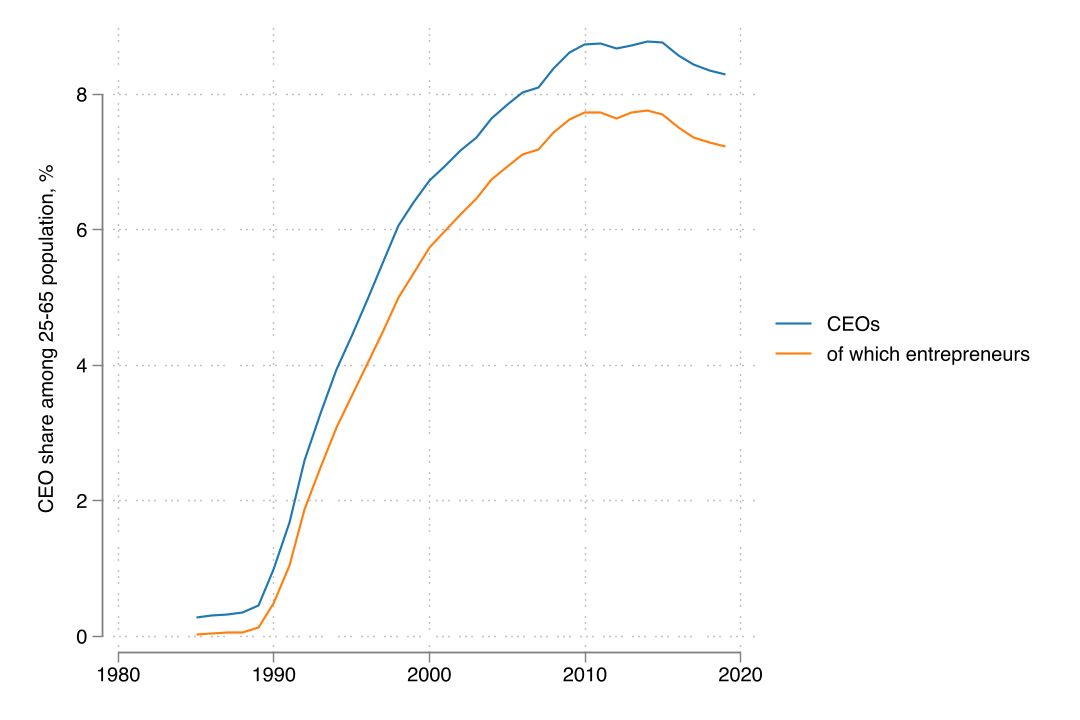
\includegraphics{fig/ceo-stock.png}
\end{frame}

\begin{frame}{The Inflow of Managers Jumped Suddenly}
\protect\hypertarget{the-inflow-of-managers-jumped-suddenly}{}
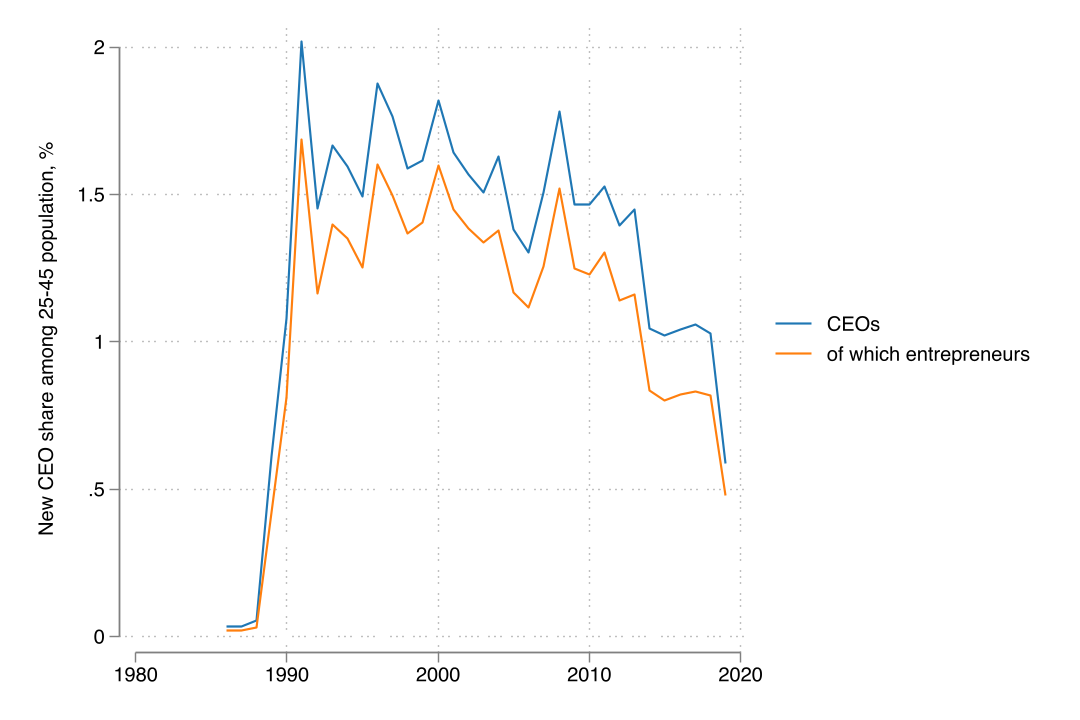
\includegraphics{fig/ceo-flow.png}
\end{frame}

\begin{frame}{Business Degrees Became More Prominent}
\protect\hypertarget{business-degrees-became-more-prominent}{}
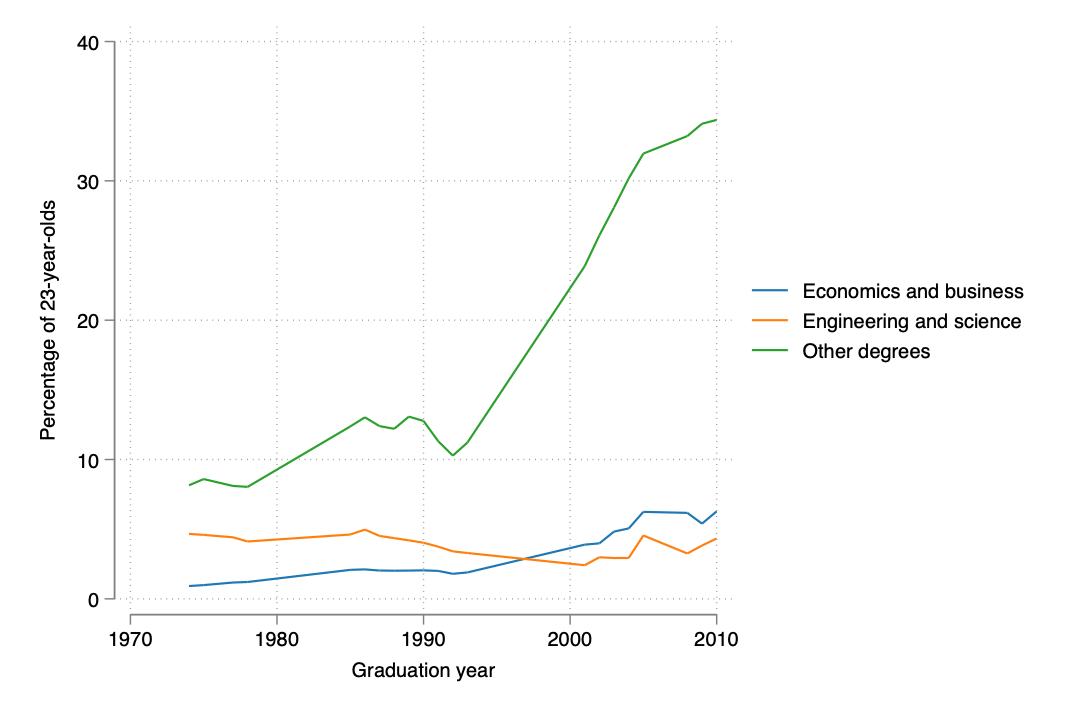
\includegraphics{fig/school-percentage.png}
\end{frame}

\begin{frame}{Large Firms are Overrepresented in Hübner}
\protect\hypertarget{large-firms-are-overrepresented-in-huxfcbner}{}
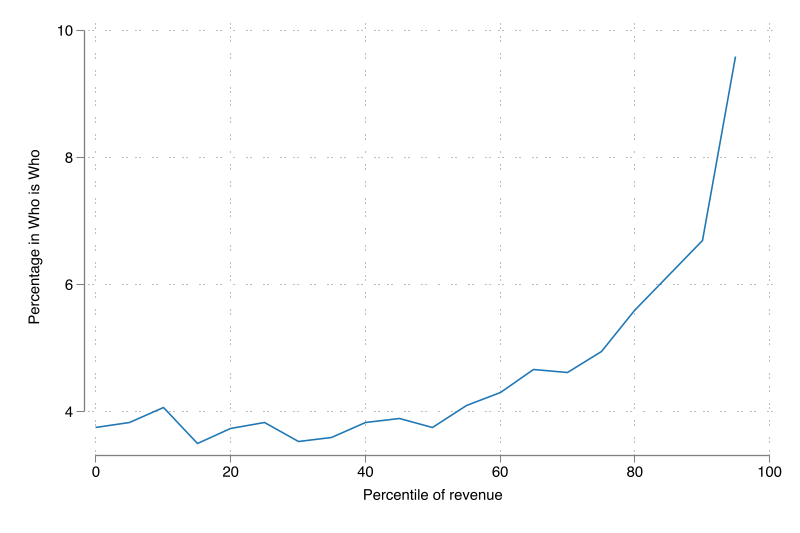
\includegraphics{fig/firm-wiw.png}
\end{frame}

\section{An OLG Model of Managers}\label{an-olg-model-of-managers}

\begin{frame}{An OLG Model of Managers}
\protect\hypertarget{an-olg-model-of-managers-1}{}
An overlapping generations model with heterogeneous manager skill,
limited span of control and career choice.

\begin{block}{Key decisions}
\protect\hypertarget{key-decisions}{}
school choice: business, engineering or other

career choice: manager or worker
\end{block}

\begin{block}{Key equilibrium feedback}
\protect\hypertarget{key-equilibrium-feedback}{}
competition within and across cohorts
\end{block}

\begin{block}{Key friction}
\protect\hypertarget{key-friction}{}
school and career choice are irreversible
\end{block}
\end{frame}

\begin{frame}{Outline}
\protect\hypertarget{outline-1}{}
\begin{enumerate}
\tightlist
\item
  Static problem: production function, input prices, competition
\item
  Manager schooling and career choice
\item
  Demographics: evolution of cohorts
\end{enumerate}
\end{frame}

\section{Static Problem}\label{static-problem}

\begin{frame}{Production Function}
\protect\hypertarget{production-function}{}
Managers differ in their innate skill level. A manager with skill \(z\)
can hire \(h\) workers to produce output with the production function
\[q = z^\nu h^{1-\nu}\] \(\nu>0\) captures span of control (Lucas 1978):
hard to run a large firm.
\end{frame}

\begin{frame}{Firm Revenue}
\protect\hypertarget{firm-revenue}{}
\[r(z) = q(z) = z w^{1-1/\nu}(1-\nu)^{1/\nu-1}\]

Employment, production wage bill, revenue, and manager wages are all
linear in \(z\).

Real wage (\(w\)) is endogenous, determined in competition with other
managers.
\end{frame}

\begin{frame}{Labor Market Clearing}
\protect\hypertarget{labor-market-clearing}{}
\[L^{p} = N w^{-1/\nu}(1-\nu)^{1/\nu}\int z dG(z)\]

With \(Z := N\int z dG(z)\) denoting the sum of all manager skills,
labor market clearing becomes
\[w  = (1-\nu)\left(\frac {L^{p}}{Z}\right)^{-\nu}\]

Aggregate GDP: \[Y = Z^\nu {L^{p}}^{1-\nu}\]
\end{frame}

\begin{frame}{Manager Wages in Equilibrium}
\protect\hypertarget{manager-wages-in-equilibrium}{}
In equilibrium, firms make zero profit. Manager wages capture all
quasi-rents.

\[\omega(z) = \nu z \left(\frac {L^{p}}{Z}\right)^{1-\nu}\] This is
increasing in \(z\) but decreasing in \(Z\). Better managers make more,
but competition from other managers reduces the wages available to each
individual manager.
\end{frame}

\section{Education and Career Choice}\label{education-and-career-choice}

\begin{frame}{Education and Career Choice}
\protect\hypertarget{education-and-career-choice-1}{}
\begin{enumerate}
\tightlist
\item
  Choose school \(i\)
\item
  Draw innate manager skill \(z\)
\item
  Get trained in school: \(z\to\lambda_i z\)
\item
  Choose whether manager or worker
\end{enumerate}

We solve the model backwards.
\end{frame}

\begin{frame}{Distribution of Manager Skills}
\protect\hypertarget{distribution-of-manager-skills}{}
We assume that \(z\) is distributed Pareto, depending on schooling
\[1-F_i(x) = \Pr(z > x|\text{school}=i) = \left(\frac x{\lambda_i z_0}\right)^{-\theta}\]
for \(\theta>1\) (so that the distribution has a finite mean).
\end{frame}

\begin{frame}{Career Choice After Graduation}
\protect\hypertarget{career-choice-after-graduation}{}
Potential managers choose to enter if net value exceeds the opportunity
cost, \[(1-\tau)v(t)z > J(t)\] Selection on manager skill,
\[z > z_{\min}(t) := \frac {J(t)} {(1-\tau)v(t)}.\]

Manager wages may be taxed at rate \(\tau\in[0,1)\).

Entry cutoff \(z_{\min}\) independent of school \(i\).
\end{frame}

\begin{frame}{Expected Career When Entering School}
\protect\hypertarget{expected-career-when-entering-school}{}
Schools affect

\begin{enumerate}
\tightlist
\item
  the probability of becoming a manager
\item
  expected skills and wages
\end{enumerate}
\end{frame}

\begin{frame}{Probability of becoming a manager}
\protect\hypertarget{probability-of-becoming-a-manager}{}
\[
\pi_i(t) = 
    z_{\min}(t)^{-\theta}
        (\lambda_i z_0)^{\theta}
\]
\end{frame}

\begin{frame}{Average manager skills}
\protect\hypertarget{average-manager-skills}{}
\[\tilde z(t) = \frac {\theta}{\theta-1} z_{\min}(t) \]
\end{frame}

\begin{frame}{Manager Value}
\protect\hypertarget{manager-value}{}
Bellman equation for manager value:
\[\rho V(t,z) = \omega[z,Z(t)] - \delta V(t,z) + V_t(t,z)\] Guess
solution: \[V(t,z) = v(t)z\] If this is the case, the Bellman can be
rewritten as
\[\rho v(t) = \nu p \left[\frac {L^{p}(t)}{Z(t)}\right]^{1-\nu} - \delta v(t) + v'(t)\]
\end{frame}

\begin{frame}{Expected labor income from a degree}
\protect\hypertarget{expected-labor-income-from-a-degree}{}
\begin{multline*}
E_i(t) = 
\pi_i(t)(1-\tau) v(t) \tilde z(t) + [1-\pi_i(t)] J(t) = \\
J(t) \left[
1 + (\lambda_i z_0)^\theta (1-\tau)^{\theta} v(t)^\theta J(t)^{-\theta}/(\theta-1)
\right]
\end{multline*}
\end{frame}

\begin{frame}{Probability of choosing school \(i\)}
\protect\hypertarget{probability-of-choosing-school-i}{}
\[
x_i = \frac {e^{\alpha_i} \left[
1 + (\lambda_i z_0)^\theta (1-\tau)^{\theta} v(t)^\theta J(t)^{-\theta}/(\theta-1)
\right]^{1/\gamma}   } 
{\sum_j e^{\alpha_j}\left[
1 + (\lambda_j z_0)^\theta (1-\tau)^{\theta} v(t)^\theta J(t)^{-\theta}/(\theta-1)
\right]^{1/\gamma}   }.
\]

\(1/\gamma\): elasticity of school choice

\(\alpha_i\): attractiveness of school \(i\)
\end{frame}

\begin{frame}{Aggregate skill level}
\protect\hypertarget{aggregate-skill-level}{}
\[
\Lambda(t) = \left[\sum_i x_i \lambda_i^\theta \right]^{1/\theta}
\]
\end{frame}

\section{Demographics}\label{demographics}

\begin{frame}{Manager and Worker Demographics}
\protect\hypertarget{manager-and-worker-demographics}{}
Workers and managers die at a constant rate \(\delta\).

The stock of population: \[
L := \int_{-\infty}^t e^{\delta{(s-t)}}l ds = l/\delta.
\] The mass of active managers: \[
N(t) := \int_{-\infty}^t e^{\delta{(s-t)}}n(s) ds.
\] The stock of workers: \[L^{p} (t) := L-N(t)\]
\end{frame}

\begin{frame}{Competition Between Firms}
\protect\hypertarget{competition-between-firms}{}
Potential new managers have a time invariant skill distribution
\(F(z)\).

Only the best become managers: a time varying truncation of \(F\).

The distribution of skill among the stock of managers, denoted by
\(G(t, z)\), is a mixture of these truncated distributions.
\end{frame}

\begin{frame}{What can policy do?}
\protect\hypertarget{what-can-policy-do}{}
\begin{enumerate}
\tightlist
\item
  Lower \(\tau\) \(\to\) more managers
\item
  Increase \(\alpha_i\) for high-\(\lambda_i\) schools \(\to\) better
  composition \(\to\) higher \(\Lambda\)
\item
  Increase \(\lambda_i\) directly \(\to\) higher \(\Lambda\) (directly
  and indirectly)
\end{enumerate}
\end{frame}

\begin{frame}{A taxonomy of macro effects}
\protect\hypertarget{a-taxonomy-of-macro-effects}{}
\begin{block}{Supply}
\protect\hypertarget{supply-1}{}
Higher \(x_i\) going to business schools
\end{block}

\begin{block}{Selection}
\protect\hypertarget{selection-1}{}
Better innate ability of managers, \emph{conditional} on school choice
\end{block}

\begin{block}{Competition}
\protect\hypertarget{competition-1}{}
Worker and manager wages respond to entry of new managers
\end{block}
\end{frame}

\begin{frame}{Dynamics}
\protect\hypertarget{dynamics}{}
Bellman equation of manager wages
\[v'(t) = (\rho+\delta) v(t) - \nu \left[\frac {L^{p}(t)}{Z(t)}\right]^{1-\nu}\]
The set of managers will be a slowly moving state variable.
\[N'(t) = n(t) - \delta N(t)\] The change in the overall skill of
managers is \[Z'(t) = n(t)\tilde z(t) - \delta Z(t)\] The change in the
discounted PV of worker wages is \[J'(t)=(\rho+\delta)J(t)-w(t)\]
\end{frame}

\begin{frame}{Dynamic Equilibrium}
\protect\hypertarget{dynamic-equilibrium}{}
Ordinary differential equations in \(Z\) and \(N\) (state) and \(v\) and
\(J\) (co-state):

\begin{align*}
v'(t) &= (\rho+\delta) v(t) - \nu \left[\frac {L - N(t)}{Z(t)}\right]^{1-\nu} \\
Z'(t) &= \frac{\theta}{\theta-1} \delta L [\Lambda(t)z_0]^\theta (1-\tau)^{\theta-1} [v(t)/J(t)]^{\theta-1} - \delta Z(t) \\
N'(t) &= \delta L [\Lambda(t)z_0]^\theta (1-\tau)^{\theta} [v(t)/J(t)]^\theta - \delta N(t) \\
J'(t) &= (\rho+\delta) J(t) - (1-\nu) \left[\frac {L - N(t)}{Z(t)}\right]^{-\nu}
\end{align*}
\end{frame}

\begin{frame}{Steady State}
\protect\hypertarget{steady-state}{}
The steady state of this economy is when
\(v'(t) = Z'(t) = N'(t) = J'(t) = 0\).

We have an almost analytical solution.

Steady state is saddle-path stable.
\end{frame}

\begin{frame}{Manager share in the steady state}
\protect\hypertarget{manager-share-in-the-steady-state}{}
\[
\frac{N_*}{L} = \frac 1{1+  
\frac {1-\nu}{(1-\tau)\nu}
\frac {\theta}{\theta - 1}}
\]
\end{frame}

\begin{frame}{GDP accounting}
\protect\hypertarget{gdp-accounting}{}
Value added per worker in the steady state: \[
\frac{Y_*}{L} = 
\left(\frac{\nu}{1-\nu} \right)^\nu
(1-\tau)^\nu
(\Lambda_* z_0)^\nu
\left(\frac {N_*}{L}
\right)^{-\nu/\theta}
\left(1-\frac {N_*}{L}
\right)
\]
\end{frame}

\begin{frame}{Predictions}
\protect\hypertarget{predictions}{}
GDP per capita is increasing in:

\begin{enumerate}
\tightlist
\item
  Innate manager skill
\item
  Average manager training
\end{enumerate}

Effect of \(\tau\) and manager share are ambiguous. There may be too
many managers.
\end{frame}

\begin{frame}{Transitional Dynamics}
\protect\hypertarget{transitional-dynamics}{}
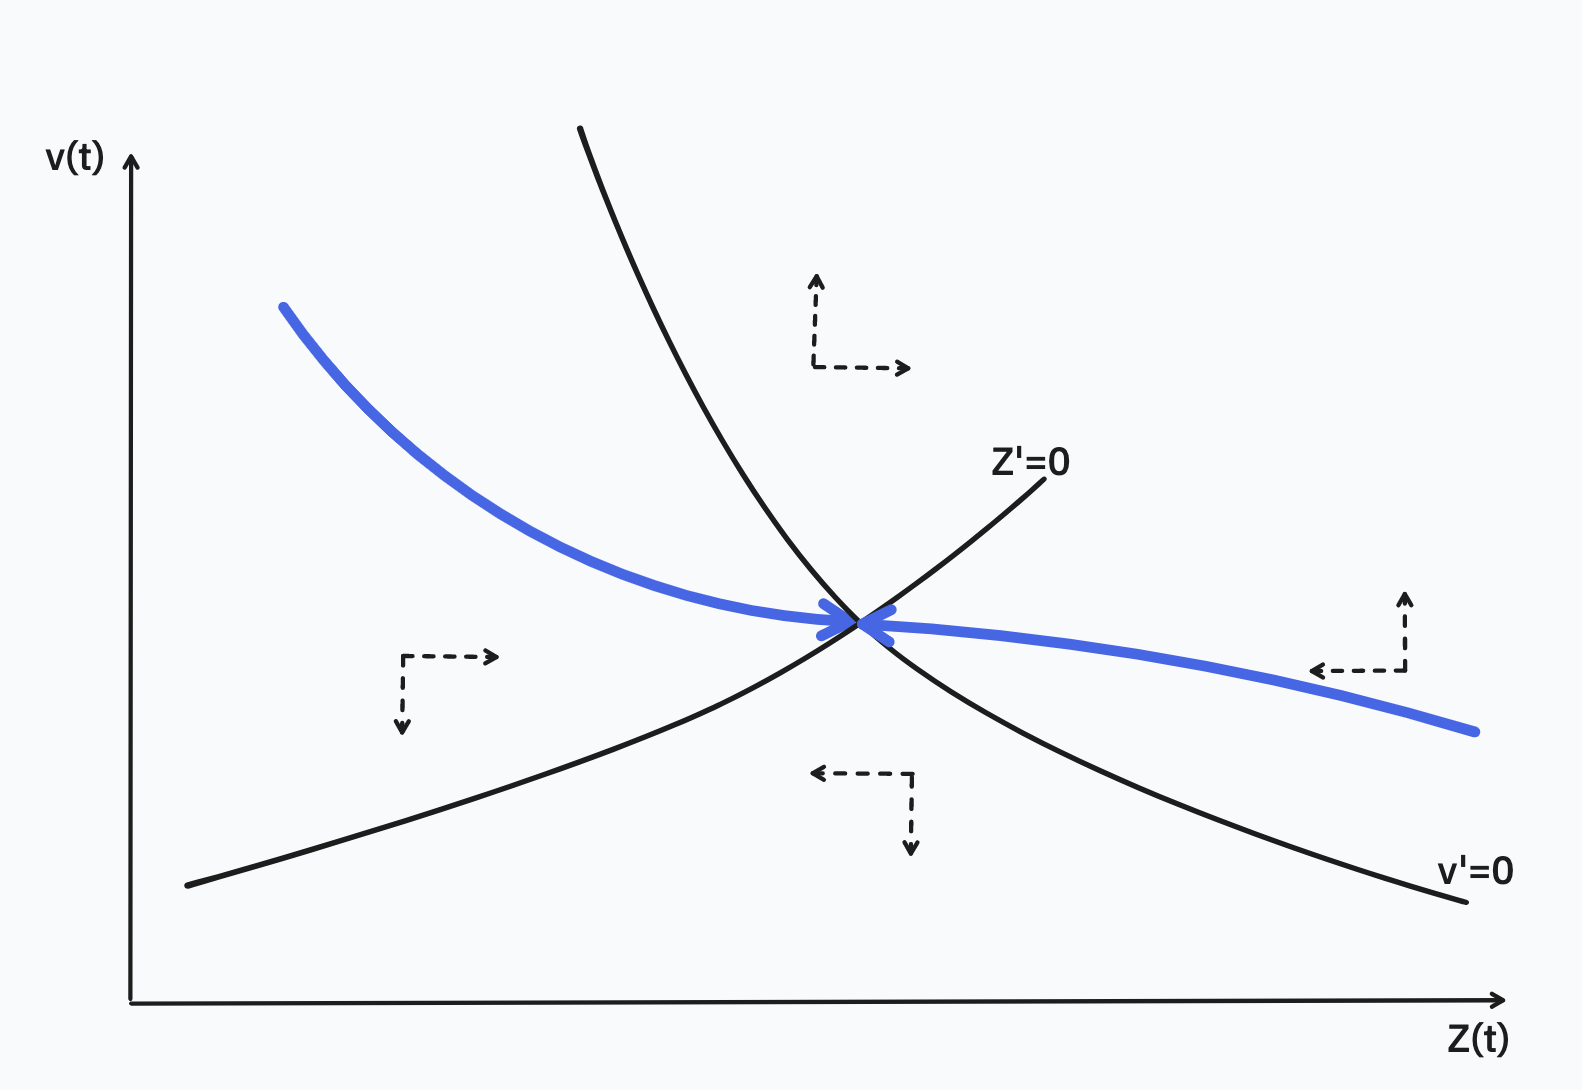
\includegraphics{fig/phase1.png}
\end{frame}

\section{Taking the Model to the
Data}\label{taking-the-model-to-the-data}

\begin{frame}{Goal}
\protect\hypertarget{goal}{}
Calibrate model to match two steady states:

\begin{enumerate}
\tightlist
\item
  communism (1985)
\item
  capitalism (2010)
\end{enumerate}

with only one change, \(\tau\to 0\).
\end{frame}

\begin{frame}{Calibration}
\protect\hypertarget{calibration}{}
\begin{table}[ht!]
\centering
\caption{Calibrated parameter values under communism}   
\begin{tabular}{clr}
  \hline
Parameter & Explanation & Value \\
    \hline
$\nu$ & Steady-state ratio of managers to workers & 0.174 \\
$\tau$ & Tax rate & 0.929 \\
$\rho$ & Discount rate & 0.050 \\
$\delta$ & Retirement rate & 0.033 \\
$\theta$ & Skill distribution, shape & 4.380 \\
$\lambda_1$ & Skill multiplier in business schools & 2.197 \\
$\lambda_2$ & Skill multiplier in engineering & 2.185 \\
$\lambda_3$ & Skill multiplier in other college & 1.649 \\
$\alpha_1$ & Relative preference for business schools & -2.23 \\
$\alpha_2$ & Relative preference for engineering & -2.02 \\
$\alpha_3$ & Relative preference for other college & -0.204 \\
$\gamma$ & Importance of non-pecuniary education benefits & 0.059 \\
    \hline
\end{tabular}
\end{table}
\end{frame}

\begin{frame}{Measuring manager quality}
\protect\hypertarget{measuring-manager-quality}{}
Log revenue of firm \(i\) in year \(t\) in industry \(s\), with a
mananager having entered in cohort \(c\) is \[
\ln R_{icst} = \beta_1\text{manager\_age}_{ict} + \beta_2\text{firm\_age}_{ict}  + \mu_{c} + \xi_{st} + \epsilon_{ict}.
\]
\end{frame}

\begin{frame}{Degree of Selection}
\protect\hypertarget{degree-of-selection}{}
\[
\ln \pi_{ic} = \theta\ln\lambda_i  - \theta \mu_c + \varepsilon_{ic}.
\]
\end{frame}

\begin{frame}{Manager Selection by Degree}
\protect\hypertarget{manager-selection-by-degree}{}
\begin{center}
\begin{tabular}{lc} \hline
 & (1) \\
VARIABLES & ln\_pi \\ \hline
\vspace{4pt} & \begin{footnotesize}\end{footnotesize} \\
(firstnm) firm\_size & -6.872*** \\
\vspace{4pt} & \begin{footnotesize}(1.982)\end{footnotesize} \\
(firstnm) degree = 1, economics & 4.032*** \\
\vspace{4pt} & \begin{footnotesize}(0.368)\end{footnotesize} \\
(firstnm) degree = 2, engineering & 3.676*** \\
\vspace{4pt} & \begin{footnotesize}(0.492)\end{footnotesize} \\
(firstnm) degree = 3, other & 2.041*** \\
\vspace{4pt} & \begin{footnotesize}(0.455)\end{footnotesize} \\
Constant & -14.92*** \\
 & \begin{footnotesize}(2.106)\end{footnotesize} \\
\vspace{4pt} & \begin{footnotesize}\end{footnotesize} \\
Observations & 87 \\
 $R^2$ & 0.553 \\ \hline
\multicolumn{2}{c}{\begin{footnotesize} Robust standard errors in parentheses\end{footnotesize}} \\
\multicolumn{2}{c}{\begin{footnotesize} *** p$<$0.01, ** p$<$0.05, * p$<$0.1\end{footnotesize}} \\
\end{tabular}
\end{center}

\end{frame}

\begin{frame}{Policy Counterfactuals}
\protect\hypertarget{policy-counterfactuals}{}
\begin{enumerate}
\tightlist
\item
  \textbf{Transition}: Reduce \(\tau\) to 0 suddenly.
\item
  \textbf{Manager tax}: Reduce \(\tau\) to increase GDP by 5 percent.
\item
  \textbf{School benefit}: Increase \(\alpha_i\) to increase GDP by 5
  percent.
\item
  \textbf{Curriculum reform}: Increase \(\lambda_i\) to increase GDP by
  5 percent.
\end{enumerate}
\end{frame}

\begin{frame}{Transition: Manager entry increases suddenly}
\protect\hypertarget{transition-manager-entry-increases-suddenly}{}
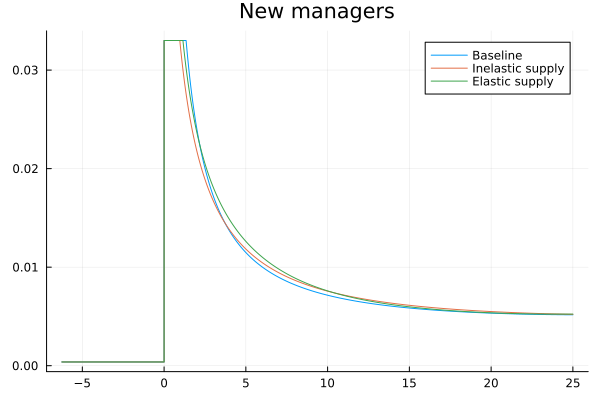
\includegraphics[width=13cm,height=8cm]{fig/model-entry-liberalization.png}
\end{frame}

\begin{frame}{Transition: Entrant skill drops sharply}
\protect\hypertarget{transition-entrant-skill-drops-sharply}{}
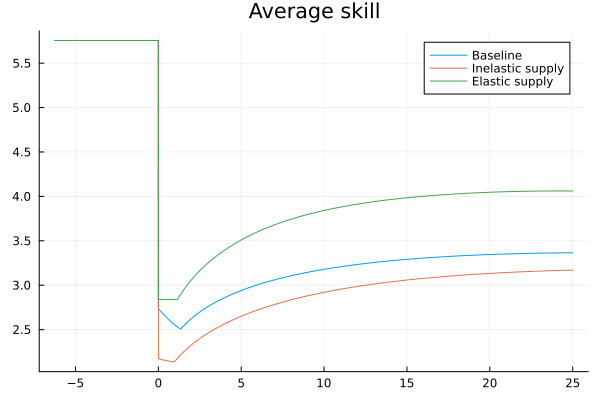
\includegraphics[width=13cm,height=8cm]{fig/model-skill-liberalization.png}
\end{frame}

\begin{frame}{Transition: Business schools become more popular}
\protect\hypertarget{transition-business-schools-become-more-popular}{}
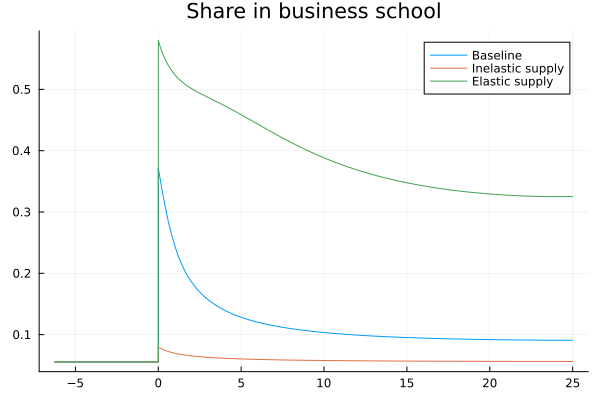
\includegraphics[width=13cm,height=8cm]{fig/model-econ-liberalization.png}
\end{frame}

\begin{frame}{Transition: GDP converges to a higher steady state}
\protect\hypertarget{transition-gdp-converges-to-a-higher-steady-state}{}
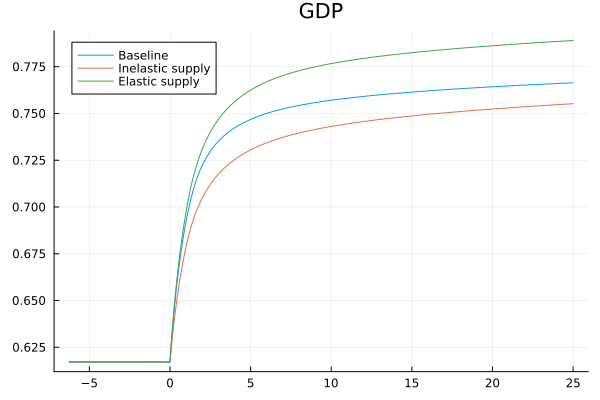
\includegraphics[width=13cm,height=8cm]{fig/model-gdp-liberalization.png}
\end{frame}

\begin{frame}{Policy Counterfactuals}
\protect\hypertarget{policy-counterfactuals-1}{}
\begin{tabular}{lcccc}
\toprule
{} & Transition ($\tau$) & Manager tax & School benefit & Curriculum \\
\midrule
Percentage change        &         -100.0 &        -3.7 &       26.7 &           47.4 \\
Manager entry            &           58.4 &         7.1 &         0.0 &            0.0 \\
Average education        &            2.3 &         0.1 &         5.0 &            5.0 \\
Selection                &           -9.5 &        -1.5 &         0.0 &            0.0 \\
Competition              &          -13.0 &        -0.6 &         0.0 &            0.0 \\
\midrule
Total GDP change         &           27.6 &         5.0 &         5.0 &            5.0 \\
\midrule
Share in business school &          10.8 &       3.6 &       61.4 &          5.5 \\
\bottomrule
\end{tabular}
\end{frame}

\begin{frame}{Discussion}
\protect\hypertarget{discussion}{}
\begin{enumerate}
\tightlist
\item
  Manager entry can increase GDP substantially. But

  \begin{itemize}
  \tightlist
  \item
    Only if starting from a very low level.
  \item
    There are large pushbacks from selection\ldots{}
  \item
    \ldots and competition.
  \end{itemize}
\item
  Subsidizing business schools has more direct effect on GDP. But

  \begin{itemize}
  \tightlist
  \item
    Requires implausibly large increase in enrollment.
  \end{itemize}
\item
  Curriculum reform has the most direct effect on GDP.
\end{enumerate}
\end{frame}

\section{Conclusion}\label{conclusion}

\begin{frame}{Conclusion}
\protect\hypertarget{conclusion-1}{}
\begin{block}{Go Corvinus!}
\protect\hypertarget{go-corvinus}{}
\end{block}
\end{frame}

\end{document}
